\section{Background}
In order to achieve Model Predictive Control, it\textquotesingle s important to build a valid model of the dynamics of the RC car. In order to do so, it\textquotesingle  s important to understand the tire characteristics of this vehicle. This means there has to be a model for the tire characteristics as well. To build such a model, Data-Driven Model Design is used. 
To analyse the data of the test rig, a dynamical model is necessary. For this case, the Bicycle Model is chosen. 
In the Bicycle Model, the car is represented as a rigid, two-dimensional, two-wheel vehicle with a xyz-coordinate system is fixed to the car frame. The front wheels are represented as one wheel and so are the rear wheels \ref{fig:bicyclemodel}.

 This model comes with some important assumptions so there are some restrictions to test settings as well. The car should not move in the vertical (z-) position, nor rotate in the roll and pitch directions (around the x- and y- axes respectively). Therefore, movements are only possible in the x- and y-direction and as a rotation around the z-axis(yaw). 
Furthermore, the bicycle model is divided in two parts: the linear and the nonlinear bicycle model. In the linear bicycle model, constant longitudinal velocity is assumed and lateral acceleration should not exceed 0.3 g . this means during testing, the vehicle is not allowed to accelerate while cornering. Also, the car can't accelerate too much while going straight otherwise it might exceed the lateral maximum of 0.3g.
\begin{figure}
	\centering
		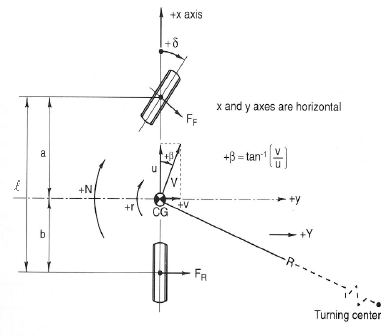
\includegraphics[scale=0.5]{figure/bicyclemodel.png}
	\label{fig:bicyclemodel}
	\caption{Bicycle model}
\end{figure}
In most cases the nonlinear bicycle model should be used. In this model, the limitations stated in the previous section will not occur. This model comes with a larger set of equations and variables, and is solvable if the distribution of forces on the front and rear tires is known. In order to solve the equations, we assume a 50-50 distribution on these wheels, which makes sense if both the front and rear wheels are spinning at the same time. Because the wheels are connected to the same motor ,through differentials, and share the same properties, the forces acting on the wheels are approximately the same.
When the forces acting on the wheels of the car are known, thanks to the bicycle model values can be found to determine the slip angle \( \alpha \)  and the slip ratio \(\kappa\) . With these known, the tire characteristics can be determined using the Magic Formula tire model \ref{eq:magicformula}. 
\begin{equation}
	[F_{xwi} ,F_{ywi}] = MF(F_{zi},\alpha_{i},\kappa_{i},\mu) (i = f,r)
	\label{eq:magicformula} 
\end{equation}


With equation \ref{eq:magicformula} with every variable known except the friction coefficient \(\mu\), the variable \(\mu\) can be determined. Then an overview is created of all the tire characteristics of the RC vehicle, which is represented in a 3D-plot.
